\section{Results}\label{sec:results}
\subsection{Information, Geometry, Cost Noise, and Generalization (RQ1)}\label{sec:rq1}
The single-bay baseline (\texttt{S1}, 7 bay positions $\times$ 60 seeds $=420$ encounters per policy) tests whether communication is necessary. Without it, \texttt{reactive} completed $93.8\%$ [91.1--95.7\%] of encounters and deadlocked in 26, when random patience timers failed to break symmetry within $180$\,s; both robots backed up together in $39\%$ of episodes. Over successes it averaged $97.1\pm4.5$\,s of total delay against $26.8\pm0.6$\,s for the reference ($3.6\times$); charging $180$\,s per robot in every deadlock raises this to $113$\,s ($4.2\times$), and its failure-charged excess $\Delta^{u}$ is $86.5$\,s. All four negotiating policies completed 420/420 encounters without collision; because \texttt{fixed\_priority} uses the broadcast protocol, its gain combines a shared tie-break with messaging. Randomized exponential backoff (\texttt{S11b}) raises completion to $96.7\%$ (\texttt{S1}) and $100\%$ (\texttt{S4}) but not efficiency ($\Delta^{u}=92.3\pm6.3$ and $59.1\pm4.0$\,s, against $6.5\pm0.6$ and $1.1\pm0.3$\,s for \texttt{fixed\_priority}). One-at-a-time sweeps of every rulebook threshold (\texttt{S11a}) changed excess delay by less than $0.8$\,s, except an urgency threshold of $2.5$ (\texttt{S2}: $3.5\to15.7$\,s for \texttt{rules\_default}, $9.1$\,s for \texttt{rules\_proximity}) and a $1.0$\,m closest-refuge tie margin, which moves \texttt{rules\_proximity} toward \texttt{rules\_default} ($3.2\to5.6$\,s in \texttt{S1}, $5.6\to3.2$\,s in \texttt{S4}).

\begin{figure}[!t]\centering
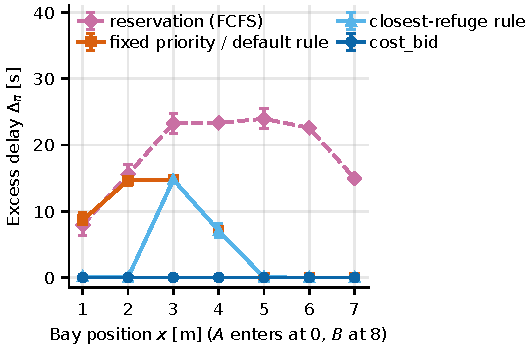
\includegraphics[width=\columnwidth]{Images/fig5_bay_geometry.pdf}
\caption{Mean excess delay $\Delta_\pi$~\eqref{eq:excess} versus pull-in bay coordinate $x$ in the single-bay corridor across negotiating policies (\texttt{S1}) and first-come corridor mutex locking (\texttt{reservation}). Error bars show 95\% CIs.}
\label{fig:rq1_geom}
\end{figure}

Efficiency then depends on how a policy exploits geometry (Fig.~\ref{fig:rq1_geom}). \texttt{fixed\_priority} and \texttt{rules\_default}, identical for equal robots because $A$ always enters first, average $\Delta^{u}=6.4\pm 0.6$\,s and peak at $14.6$--$14.8$\,s when the bay sits near $A$'s entrance and $B$ must reverse to \texttt{room\_hi}. Ranking proximity ahead of seniority (\texttt{rules\_proximity}) halves this to $3.1\pm 0.5$\,s. The advantage is layout-specific: with two bays (\texttt{S4}, 360 encounters), \texttt{rules\_proximity} incurs $5.6\pm 0.5$\,s and picks the reference yielder in only $14\%$ of encounters, worse than \texttt{fixed\_priority} ($1.1\pm 0.3$\,s) and \texttt{rules\_default} ($1.2\pm 0.3$\,s), which are equivalent within $\pm0.5$\,s (paired $+0.14$\,s, TOST $p<0.001$). First-come \texttt{reservation} (210 encounters) never deadlocked but incurred $18.8\pm 0.9$\,s, three times \texttt{fixed\_priority} on the same draws, because $B$ starts on $A$'s exit path and must park inside \texttt{room\_hi} while $A$ traverses the whole aisle. A layout with staging off the exit path could not be tested: parking $1.2$\,m or more deeper in the end room made every episode deadlock under the current leave maneuver. Noise-free \cb\ chose the reference yielder in every \texttt{S1} and \texttt{S4} encounter; since it uses the simulator's true speed limits, this mainly validates the cost model. Its mean absolute prediction error is $1.9$\,s per robot, and predicted delay is on average $15\%$ below realized delay, a bias common to both outcomes; the residual scatter, the SD of $\log(\text{predicted}/\text{realized})$, is $0.075$ (\texttt{S1}) and $0.068$ (\texttt{S2}).

In mixed fleets (\texttt{S2}, 5,040 episodes, Supplementary Fig.~S8; $u_B\in\{1,3\}$, payload, $v_B\in\{0.26,0.13\}$\,m/s), \texttt{fixed\_priority} incurs $\Delta^{w}=27.1\pm 2.6$\,s because it sends urgent, loaded, or slow robots into long reversals. \texttt{rules\_default} cuts this to $3.5\pm 0.4$\,s, while the reference that minimizes \emph{unweighted} delay still incurs $7.0\pm 1.5$\,s: optimizing the wrong objective costs twice as much as replacing the planner with a rulebook. Weighted \cb\ reaches $0.04\pm 0.02$\,s, matching the weighted reference's yielder in $98\%$ of encounters; the 16 misses are near-ties (median bid gap $0.6$\,s).

\begin{table}[!t]\centering
\caption{Paired excess-delay difference of noisy \cb\ minus a rulebook on the same draws (s; stratified bootstrap 95\% CI). Negative favors \cb. Single bay: vs.\ \texttt{rules\_proximity}, $\Delta^{u}$, 210 draws per $\sigma$ (\texttt{S7d}); heterogeneous: vs.\ \texttt{rules\_default}, $\Delta^{w}$, 720 draws (\texttt{S7h}).}
\label{tab:sigma}
{\footnotesize\setlength{\tabcolsep}{4pt}
\begin{tabular}{@{}rrr@{}}\toprule
$\sigma$ & Single bay & Heterogeneous \\\midrule
0.10 & $-2.97$ [$-3.22$, $-2.72$] & $-3.15$ [$-3.33$, $-2.96$] \\
0.25 & $-1.45$ [$-2.06$, $-0.81$] & $-1.94$ [$-2.23$, $-1.64$] \\
0.30 & $-0.85$ [$-1.51$, $-0.15$] & $-1.46$ [$-1.79$, $-1.11$] \\
0.35 & $-0.21$ [$-0.99$, $+0.58$] & $-0.89$ [$-1.33$, $-0.41$] \\
0.40 & $+0.39$ [$-0.46$, $+1.30$] & $-0.30$ [$-0.86$, $+0.31$] \\
0.45 & $+0.76$ [$-0.13$, $+1.65$] & $+0.00$ [$-0.59$, $+0.63$] \\
0.50 & $+1.01$ [$+0.12$, $+1.91$] & $+0.08$ [$-0.55$, $+0.75$] \\
0.75 & $+1.84$ [$+0.89$, $+2.83$] & $+4.36$ [$+3.13$, $+5.66$] \\
1.00 & $+2.34$ [$+1.34$, $+3.30$] & $+6.09$ [$+4.66$, $+7.51$] \\\bottomrule
\end{tabular}}
\end{table}

Real robots predict delays only approximately. Multiplying each robot's bid by independent log-normal noise $e^{\sigma\epsilon}$ (Table~\ref{tab:sigma}), \cb\ is significantly better than \texttt{rules\_proximity} in the single bay up to $\sigma=0.3$, tied at $0.35$--$0.45$, and worse from $0.5$ (\texttt{S7d}; the original five-point \texttt{S7} grid in Supplementary Fig.~S1 agrees). In heterogeneous fleets (\texttt{S7h}) it beats both rulebooks up to $\sigma=0.35$, ties at $0.4$--$0.5$, and is worse from $0.75$, while \texttt{fixed\_priority} stays $17$--$27$\,s worse; keying the noise on the decision time instead of the episode moves this tie point to $\sigma=0.5$. Systematic error matters little: mis-specifying reverse speed and turn rate by $\pm10$--$30\%$ for one or both robots (\texttt{S7m}) raised \cb\ excess by at most $0.2$\,s, because a shared bias shifts both outcomes alike. The planner's measured scatter ($\sigma\approx0.07$ in 2D; $0.095$ in Gazebo against $0.098$ in 2D on the same 72 nominal two-robot runs) lies well inside the region where bidding wins, but hardware error is untested, and these single-bay crossovers should not be carried to multi-bay layouts, where \texttt{rules\_proximity} trails fixed priority.

A planner-free classifier (\texttt{learned}; Supplementary Sec.~S-II) matches \texttt{rules\_default} on 150 held-out encounters of its two-bay training layout ($\Delta^{w}=+2.6\pm1.1$ vs.\ $+2.5\pm1.0$\,s), but on an unseen single-bay layout it reaches $+13.1\pm4.1$\,s, no better than \texttt{fixed\_priority} ($+12.3\pm3.4$\,s). Only $15\%$ of those encounters hit unseen keys, and seen keys err as much ($+13.6\pm4.6$\,s): the coarse bins encode layout-specific outcomes. We treat this as an illustration of the generalization risk of tabular lookups, not an evaluation of learned coordination.

\subsection{Strategic Incentives and Repeated-Encounter Fairness (RQ2)}\label{sec:rq2}
Self-interested robots can exaggerate delays to avoid yielding. In \texttt{S6} (1,080 episodes; lower bid yields, no payment), $B$ forces $A$ to yield in every encounter by scaling its bid by $k\ge 2$, cutting its own delay from $9.1\pm 1.4$ to $8.1\pm 1.2$\,s while fleet delay rises by $4.9$\,s ($+20\%$). In the unpriced arm of \texttt{S9} (Fig.~\ref{fig:rq2_misreport}), $A$ gains up to $+4.74\pm 0.99$\,s by inflating fourfold; the asymmetry reflects roles, since truthful bidding makes $A$ yield in $67\%$ of encounters and $B$ in $33\%$. Making the proceeder pay the yielder's bid reverses the incentive: $A$ gains $+7.54\pm 1.76$\,s by under-reporting at $k=0.25$.

\begin{figure}[!t]\centering
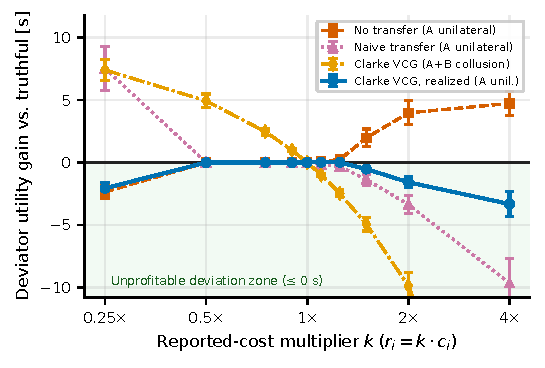
\includegraphics[width=\columnwidth]{Images/fig9_strategic_misreport.pdf}
\caption{Deviator single-encounter utility gain (seconds of urgency-weighted delay plus transfer) relative to truthful reporting ($k=1\times$) across $N=10{,}080$ episodes in \texttt{S9}; values $\le 0$\,s (shaded green) indicate unprofitable deviations. Error bars show 95\% CIs.}
\label{fig:rq2_misreport}
\end{figure}

The Clarke-pivot mechanism (Eq.~\eqref{eq:clarke}; \texttt{S9}: 6 bay and urgency settings, deviator $\in\{A, B, AB\}$, nine scales $k\in[0.25,4]$, 60 seeds, 10,080 episodes) leaves no single-robot misreport profitable under predicted costs ($0/108$ conditions); under realized travel times, lying costs $A$ up to $3.3\pm 1.0$\,s and $B$ up to $4.9\pm 1.2$\,s, and the largest gain is $+0.02\pm 0.02$\,s. Because both types come from shared snapshots, this is an implementation check, not evidence of robustness to private information. \texttt{S9b} therefore treats urgency $u_i$ as private and lets the deviator misreport it or scale $b_i(A)$ and $b_i(B)$ independently (10,080 deviating episodes): no deviation improved predicted utility, and the 89 episodes ($0.9\%$) with realized gains above $0.01$\,s all stem from execution departing from the plan, with negative mean realized gain in every arm. Payments are delay credit paid into an operator ledger, and utility is urgency-weighted delay plus payment. Three limitations remain. The ledger collects a surplus~\cite{green1977characterization} of $9.3\pm 1.6$\,s per encounter at $u_B=1$ and $10.5\pm 1.5$\,s at $u_B=3$ ($37\%$ and $24\%$ of realized weighted delay) that the operator must redistribute outside the loop. Joint shading by $k<1$ keeps $o^\ast$ but shrinks both payments, gaining $+4.94\pm 0.55$\,s at $k=0.5$ and $+7.42$\,s at $k=0.25$. And participation must be mandated: against \texttt{fixed\_priority}, $A$ loses $9.3$--$10.5$\,s per encounter, while VCG does not stop robots from hiding bays or spoofing IDs.

\begin{figure}[!t]\centering
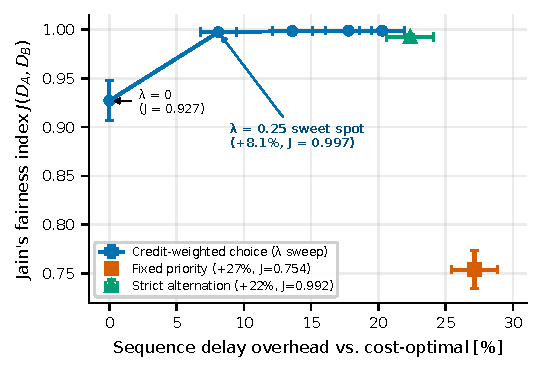
\includegraphics[width=\columnwidth]{Images/fig10_fairness_pareto.pdf}
\caption{Repeated-encounter Pareto frontier (\texttt{S10}, 50 sequences of 20 encounters) trading sequence delay overhead against cumulative Jain fairness $J(D_A^{\mathrm{cum}}, D_B^{\mathrm{cum}})$ as credit weight $\lambda$~\eqref{eq:karma} varies from $0$ to $2.0$. Error bars show 95\% CIs.}
\label{fig:rq2_fairness}
\end{figure}

Cooperative fleets need no payments, but repeated encounters can burden one robot. Over 50 sequences of 20 single-bay encounters (\texttt{S10}, Fig.~\ref{fig:rq2_fairness}), Jain's index $J$ is computed per sequence from cumulative delays and averaged; for two robots $J\in[0.5,1]$, so we also give the mean gap $|D_A - D_B|$. \texttt{fixed\_priority} gives $J=0.754$ (gap $372$\,s) at $+27.1\%$ delay over cost-optimal selection, which itself reaches $J=0.927$ (gap $128$\,s); strict turn-taking gives $J=0.992$ (gap $47$\,s) at $+22.3\%$. Choosing $\lambda$ in Eq.~\eqref{eq:karma} on these sequences (smallest overhead with $J\ge0.99$: $\lambda=0.1$) and evaluating on 100 fresh sequences (\texttt{S10b}) yields $J=0.992\pm0.002$ at $+3.8\pm0.6\%$ delay, rising to $+7.1\%$, $+11.5\%$, and $+15.7\%$ with delay-estimate error $\sigma=0.25$, $0.5$, and $1.0$ ($J\ge0.986$); the balance form selects $\lambda=0.25$ ($J=0.994$, $+3.0\%$). The fairness ledger is separate from Clarke payments, since carrying VCG credit across encounters would break single-encounter truthfulness.

\subsection{Channel Impairment, Safeguard Ablation, and Map Uncertainty (RQ3)}\label{sec:rq3}
Under moderate and heavy impairment (\texttt{S3}: loss $0$--$90\%$, latency $0.05$--$2$\,s, 3,600 episodes; \texttt{S8}: $R_{\mathrm{det}}\in\{6,3,1.5\}$\,m, $v_{\max}\in\{0.26,0.5\}$\,m/s, 4,320 episodes), every negotiating policy completed $\ge 99.3\%$ of encounters without collision (Fig.~\ref{fig:rq3_comms}); delay stayed within $1$--$2$\,s up to $50\%$ loss because \texttt{BID}s resent every $0.3$\,s arrive before the robots meet (median 664--720 messages per episode across loss levels, mostly 5\,Hz \texttt{STATE} beacons). Completion overstates negotiation, however: at the extreme loss of \texttt{S8b}/\texttt{S8c}, $62.8\%$ of episodes recorded no negotiated decision and were resolved by the reactive fallback. On fresh seeds and unseen loss levels with correlated loss (\texttt{S8d}, 2,560 episodes; Gilbert--Elliott bursts of mean length 5--100 messages, blackouts of 10--40\,s), no collision occurred and $\ge 99.4\%$ completed, but only $71.9\%$ of bursty and $92.5\%$ of blackout episodes negotiated (i.i.d.\ loss at the same mean rates: $86.7\%$). In \texttt{S8b} ($90$--$99\%$ loss, $2$--$8$\,s latency), an early agent version collided 6 times when both robots yielded on mismatched snapshots; tightened lane-clearance and bay-exit checks removed all collisions on those (development) seeds.

\begin{figure}[!t]\centering
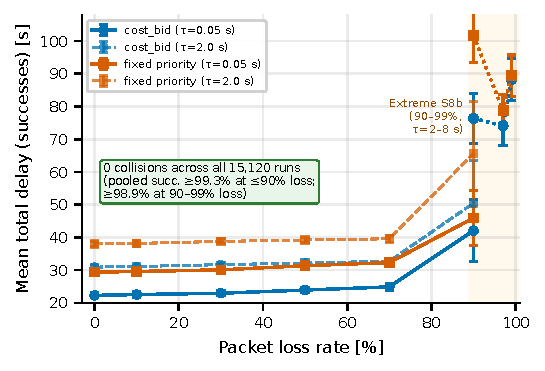
\includegraphics[width=\columnwidth]{Images/fig11_comms_resilience.pdf}
\caption{Mean total delay over successful episodes across packet loss $0$--$99\%$ and base latency $\tau\in[0.05, 8.0]$\,s (\texttt{S3} at $0.26$\,m/s and extreme \texttt{S8b} shaded right at $0.50$\,m/s); zero collisions occurred across all 15,120 communication-sweep and ablation episodes. Error bars show 95\% CIs.}
\label{fig:rq3_comms}
\end{figure}

The factorial ablation \texttt{S8c} (5,760 episodes; Supplementary Table~S-III) found no collision in any arm, even with \texttt{commit}, \texttt{state\_guard}, and \texttt{bay\_check} all off (Wilson upper bound $1.06\%$ per arm). \texttt{STATE} freshness is timed from receipt, so at 5\,Hz and $90$--$99\%$ loss a robot lacks a fresh peer message $0.90^5=59\%$ to $0.99^5=95\%$ of the time, and what it holds is $2$--$8$\,s old; collisions are prevented by the local Lidar stop and the $U[6,12]$\,s exit timer, not the radio safeguards, and \texttt{bay\_check} never triggered. \texttt{commit} added $3.1$--$3.8$\,s and raised simultaneous yields from $15$--$16\%$ to $22$--$24\%$ under \texttt{fixed\_priority}, since lost confirmations push robots past the negotiation timeout; such mutual yields have no bound on resolution time, and the 1--7 deadlocks per 360-episode arm are those outlasting $180$\,s.

With mismatched bay knowledge (two bays, 840 episodes, 10 seeds per condition), extra delay arises only when $A$ has the poorer map: knowing only \texttt{bay0}, \cb\ loses $9.1$\,s and \texttt{fixed\_priority} and \texttt{rules\_default} $29.6$\,s, as $B$ is sent to \texttt{room\_hi}. Without map sharing, decisions disagree in 109 of 420 episodes with \texttt{commit} off (7 deadlocks) and are reconciled toward the lower-ID robot with \texttt{commit} on. \texttt{share\_map} removes both the disagreements and the delay, with or without \texttt{commit} and at up to $50\%$ loss, so \texttt{commit} is needed only without map sharing. A bay blocked by an unmapped obstacle (320 episodes) deadlocked the naive \texttt{bay\_check} in $10/10$ runs; cross-checking Lidar against peer \texttt{STATE} (\texttt{refuge\_blocked}) restored $10/10$ completion ($+46$\,s when the useful bay is blocked), whereas \texttt{reactive} still deadlocked in $2/10$ and $3/10$ runs. With bays discovered while driving (\texttt{explore}; Supplementary Sec.~S-III), gating map exchange on Lidar peer detection fails at $R_{\mathrm{det}}=6$\,m because the decision precedes Lidar contact ($0/30$ maps shared; $+29.2$\,s for the rules, $+8.8$\,s for \cb), whereas \texttt{share\_map} costs nothing.

\subsection{Three-Robot Topologies and Sim-to-3D Gazebo Transfer (RQ4)}\label{sec:rq4}
In the 2-vs.-1 convoy (1,080 episodes; 72 per policy and $B$-type cell, pooling 3 seeds and $0$/$50\%$ loss; Supplementary Fig.~S9), pairwise yielding traps a reversing leader against its follower; \texttt{make\_room} removes all deadlocks ($72/72$ for every policy). \texttt{rules\_default} is the worst negotiating policy in every regime ($40.0$, $100.1$, and $133.6$\,s weighted with equal, loaded, and urgent $B$, against $33.7$, $33.7$, and $90.3$\,s for \texttt{fixed\_priority}), because its urgency and payload tiers always make the convoy yield. With equal robots ($u=1$, unloaded), pairwise \cb\ ignores the follower ($55.6$\,s), while \gb\ reaches $34.4$\,s, $+0.7\pm1.4$\,s from both \texttt{fixed\_priority} and \texttt{side\_oracle}, which coincide here. With urgent $B$, \gb\ ($104.7\pm6.7$\,s) beats \cb\ by $12.4\pm5.8$\,s but trails \texttt{fixed\_priority} by $14.4\pm8.0$\,s and \texttt{side\_oracle} by $19.0\pm6.9$\,s (\texttt{fixed\_priority} trails \texttt{side\_oracle} by $4.6\pm2.6$\,s), because Eq.~\eqref{eq:groupbid} adds member delays instead of modeling the serial wait while $C$ reverses. At the T-junction turn-in (384 episodes; 48 per policy and loss level; Supplementary Fig.~S4), waiting in the main corridor deadlocked \texttt{fixed\_priority} in $19/48$ runs; \texttt{goal\_wait} raised completion to $48/48$ at $0\%$ and $50\%$ loss for \texttt{fixed\_priority}, \texttt{rules\_default}, and \cb\ ($28/48$ for \texttt{reactive}), with delays of $60.5\pm4.7$, $53.1\pm5.0$, and $48.9\pm4.0$\,s.

\begin{table}[!t]\centering
\caption{Seed-paired ROS~2 Jazzy / Gazebo Harmonic transfer summary (460 main runs, all on the final code, plus 36 hold-batch runs; ground-truth localization).}
\label{tab:gz}
{\footnotesize\setlength{\tabcolsep}{3.0pt}
\begin{tabular}{@{}lrrrrr@{}}\toprule
Scenario / Study Group & Runs & Succ. & Coll. & Same & $\Delta D$ [s] \\\midrule
Single bay, negotiating (\texttt{S1}, S, L) & 70 & 70 & 0 & 70 & $-0.4$ \\
Single bay, \texttt{reactive}               & 10 &  9 & 1 &  5 & $-1.5$ \\
Forced yielders, S1 + S2 (O)             & 44 & 44 & 0 & 44 & $-0.5$ \\
Asymmetric urgency / speed (\texttt{S2}, neg.)    & 36 & 36 & 0 & 36 & $-0.6$ \\
Two bays (\texttt{S4})                      & 30 & 30 & 0 & 30 & $-0.2$ \\
Noisy bids ($\sigma=0.5, 1.0$; \texttt{S7}) & 12 & 12 & 0 &  7 & $+2.2$ \\
Clarke VCG misreports (\texttt{S9})         & 18 & 18 & 0 & 18 & $-0.3$ \\
50\% loss, $0.5$\,s latency (\texttt{S3})   & 18 & 18 & 0 & 18 & $-0.8$ \\
90\% loss, $2.0$\,s latency (\texttt{S8b/c})& 24 & 24 & 0 & 18 & $+4.8$ \\
Convoy 2 vs.\ 1 (\texttt{make\_room})       & 36 & 36 & 0 & 36 & $-0.6$ \\
T-junction (18 exit + 18 turn-in)           & 36 & 36 & 0 & 35 & $-16.8$ \\
Asymmetric static maps                      & 24 & 24 & 0 & 24 & $-0.3$ \\
Physically blocked bay                      & 18 & 18 & 0 & 18 & $-1.2$ \\
Explore (base, $R_{\mathrm{det}}\in\{6,3.5\}$) & 84 & 84 & 0 & 83 & $+0.2$ \\\midrule
\emph{Batch 2:} \texttt{hold\_for\_map}     & 24 & 24 & 0 & 24 & $+10.0$ \\
\emph{Batch 2:} \texttt{det\_3.5} rerun     & 12 & 12 & 0 & 11 & $+3.4$ \\\bottomrule
\end{tabular}}\\[2pt]
{\footnotesize Same: identical first yielder to paired 2D run (fixed by construction on forced runs). $\Delta D$: mean Gazebo minus 2D urgency-weighted delay over paired successes.}
\end{table}

Transfer to 3D physics, wall-filtered \texttt{LaserScan} perception, and asynchronous ROS~2 messaging\label{sec:gz} was tested in 460 main Gazebo runs covering every study (6--10 seeds per condition, $\sim5$\,min per run) and 36 hold runs, each paired with a 2D run on the same seed (Table~\ref{tab:gz}). All nodes read ground-truth pose. The 338 runs of the final release and the hold runs used an amd64 image; the 122 original single-bay, convoy, T-junction, and communication cases were rerun on the same final code on an ARM64 image, reproducing every negotiating first yielder with makespan changes of at most $1.6$\,s. Gazebo recorded no deadlock or collision in the 450 non-reactive main runs (Wilson upper bound $0.85\%$) or the hold runs, against 1 collision and 3 deadlocks in 10 \texttt{reactive} runs. Of the 406 negotiating main runs, 394 ($97.0\%$, Wilson [94.9, 98.3]\%) chose the same first yielder as in 2D; 11 of the 12 disagreements involve randomness the simulators do not share (5 noisy-bid runs, whose noise is seeded on \texttt{round(t,1)}, and 6 runs at $90\%$ loss). The 366 straight-corridor runs with identical draws (all main runs except 10 \texttt{reactive}, 12 noisy-bid, 36 convoy, and 36 T-junction runs) lie close to $y=x$ (Fig.~\ref{fig:rq4_gz_scatter}). Over the 456 runs successful in both simulators, the Gazebo-minus-2D bias is $-1.35$\,s with limits of agreement $-27.6$ to $+24.9$\,s (Supplementary Table~S-IV, Fig.~S6), and single-bay and \texttt{S2} excess delays match within $1.0$\,s for every policy.

\begin{figure}[!t]\centering
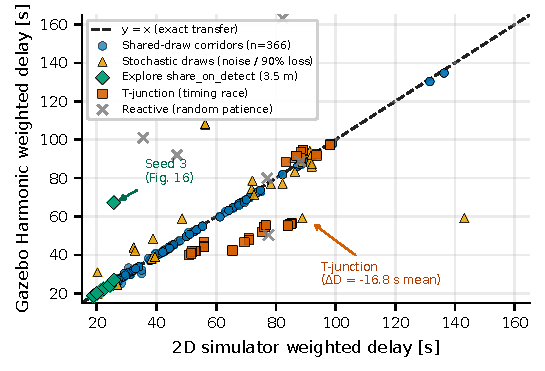
\includegraphics[width=\columnwidth]{Images/fig15_gazebo_scatter.pdf}
\caption{Paired Gazebo versus 2D urgency-weighted delay over the 460 main runs. Blue: the 366 straight-corridor runs with identical random draws; the largest departures are T-junction runs and $3.5$\,m \texttt{share\_on\_detect}.}
\label{fig:rq4_gz_scatter}
\end{figure}

Gazebo also exposed three limits invisible in 2D (Supplementary Sec.~S-IV). Wall-filtered Lidar clustering registers an oncoming Waffle only at $2.3$--$2.6$\,m, against $3.4$\,m in \texttt{sim2d}, so \texttt{share\_on\_detect} delivered no map before the decision even at $R_{\mathrm{det}}=3.5$\,m ($0/6$ runs), and \texttt{hold\_for\_map} worked only by delaying the decision ($+10.0$\,s); \texttt{share\_map} avoids the lag. Side-branch walls occlude a parked branch robot's view of the main aisle, which fusing fresh \texttt{STATE} into lane-clearance checks fixed, so the T-junction runs verify a fix rather than test blind transfer. And T-junction delays do not transfer: Gazebo accumulated $605$\,s less delay than 2D over 36 runs, partly from a release-timing race in the exit variant, while the turn-in gap ($9.5$--$28.9$\,s per run) persisted on the final code and remains unexplained.
